\documentclass{article}

\title{Failure prediction for APU's on a Metro System}
\author{Aaryadev Ghosalkar}
\date{\today}

\usepackage{algorithm}
\usepackage{algpseudocode}

\usepackage{graphicx}
\graphicspath{ {./} }
\usepackage{amsmath,amssymb}

\usepackage{tikz}
\usetikzlibrary{shapes.geometric, positioning}

\usepackage{wrapfig}

\begin{document}

\begin{titlepage}
    \begin{center}
        \vspace*{1cm}
            
        \Huge
        \textbf{Failure prediction for APU's on a Metro System}
            
        \vspace{0.5cm}
        \LARGE
        Created under Guidance of Prof. Tausif Saikh
            
        \vspace{1.5cm}
            
        \textbf{Aaryadev Ghosalkar}
            
        \vfill
            
        A Research project presented for \\
        Post Graduate Diploma in\\
        Data Science and AI
            
        \vspace{0.8cm}
            
        \Large
        Department of Technology\\
        Savitribai Phule Pune University\\
        India\\
        \today
            
    \end{center}
\end{titlepage}


\maketitle

\begin{abstract}
Predictive maintenance is vital for ensuring the reliable operation of metro transportation systems, enhancing passenger safety, and minimizing service disruptions. In this research, we focus on the challenging task of predicting failures on the Air Processing Unit (APU) on a metro system at least two hours in advance. An APU is a component on the metro responsible for compressing and storing compressed air for use on various functions on the metro such as the suspension. Our study encompasses a comprehensive comparison of various machine learning and deep learning (DL) models, including Support Vector Machines (SVM), Decision Trees, Long Short-Term Memory (LSTM) networks. These models are evaluated on the MetroPT Dataset published by Veloso et al. in 2022\cite{Veloso2022} for their performance in predicting impending failures using various metrics such as accuracy, precision, recall and F1-Score for classification, providing valuable insights into their applicability in this context.\\

Additionally, we introduce a practical demonstration of a web API designed to showcase how the model would be deployed in a real world situation. This API serves as a testament to the feasibility of deploying predictive maintenance models in production settings. \\

It is important to note that while our research offers valuable insights into model performance and deployment readiness, we refrain from proposing a final production model. This limitation arises from the complex domain knowledge required for selecting an optimal model and the to keep the paper more general since the requirements of various transportation companies need not be the same. Nevertheless, our findings contribute to the ongoing efforts to bolster metro system reliability and safety through proactive failure prediction. \\

\textbf{Keywords:} Metro system, predictive maintenance, failure prediction, machine learning, deep learning, model deployment.
\end{abstract}

\newpage

\tableofcontents

\newpage

\listoffigures
\listoftables
\listofalgorithms

\newpage

\section {Introduction}

Metro systems are a relatively new transportation solution in India, offering
passengers a convenient and efficient mode of travel. However, like any infrastructure, metro systems encounter technical faults and maintenance problems.
These issues can lead to the temporary suspension of metro services, causing
distress to commuters and operational hiccups. We don’t aim to eradicate the necessity of maintenance. Instead, our focus is on harnessing the potential of ML and DL technologies to predict when the APU on a metro is about to fail. Our inspiration comes from the
realm of existing research, which has delved into the application of AI methodologies in various engineering domains, including wind turbines and jet engines.
While the practical deployment of such systems in real-world scenarios may differ, In this study we aim to adapt and test these approaches on the MetroPT dataset and compare their applicability for predicting APU failures. This approach has the promise of
substantial cost savings by eliminating the superfluous expenses incurred during
routine system operation. Moreover, our predictive maintenance system lays the
groundwork for proactive planning. It enables us to forecast maintenance necessities well in advance.
Our Research focuses on detecting failures specifically in the Air Production Unit (APU). The APU is a vital component on any modern metro systems it is used for producing and storing compressed air for use throughout the metro system, in other components such as the air breaks and also the pneumatic
doors.

\section{Literature Review}

The initial phase of data extraction was
undertaken by the work conducted by Veloloso et al \cite{Veloso2022}. In their work they explained the operational principles of diverse sensors
and articulated the central objective of predicting metro system failures. 
Moreover, they explained the precise criteria stipulated by the railway company for the assessment of the predictive model, thus serving as an instrumental starting point for the subsequent research endeavor. \\

The findings of Azure ML Team at Microsoft \cite{AzureML2015}, show that there exist two primary approaches to tackle our problem: binary classification or failure prediction, where the objective is to predict whether the metro system will fail within the next two hours (yes or no), and regression, which in the context of our research pertains to predicting the number of cycles or amount of time before the metro system experiences a failure, or needs to be repaired. Also known as Remaining Useful life (RUL) Prediction. This paper will undertake a comparative analysis of both these approaches. \\

Davari et al \cite{Davari2021} have conducted a survey on data-driven or Machine Learning (ML) and Deep Learning (DL) approaches to PdM. In their work they have compared both approaches to we will expand on this by providing more insight into which approaches are viable in the context for metro systems.

\subsection{Failure Prediction}

Numerous traditional ML algorithms are applied in the realm of failure prediction. As detailed in the works of Chaudhuri et al \cite{chaudhuri2018}, where Support Vector Machines (SVM) and various SVM variants were employed to classify vehicles into three distinct risk categories: Immediate, Long-term, and Medium-term. This approach is simple and the results are easy to understand. \\

Convolution Neural Networks (CNN) can be applied to time series data, typically used for
images, requires a method for converting time series into image-like representations using GAF (Gramian Angular Field) feature transformation, which facilitates the conversion of one-dimensional time series data into images. Leveraging this transformation for PdM Silva reported an accuracy rate of 93\% on the SF103 dataset \cite{Silva2019}. \\

Long Short-Term Memory (LSTM) networks have gained prominence for failure prediction. Nguyen and Medjaher employed LSTM to predict failures by quantifying the probability of system failure within a specified time window \cite{nguyen2019}. This approach holds promise for our problem, as it not only offers the potential for interpretability but also grants flexibility to the company in defining the severity thresholds for failure prediction.

\subsection{Remaining Useful Life Estimation}

An alternative perspective on the problem involves estimating the Remaining Useful Life (RUL), which offers a versatile approach. This approach allows for the setting of thresholds to define significant risk levels based on the transportation companies needs this is usually done by monitoring specific variables that serve as reliable indicators of system deterioration however this approach requires domain knowledge about the features that can be used to predict the degradation of the system, since we do not know any features which could be used for this we recommend taking a slightly different approach by calculating the number of hours to failure see section 3.2. \\

Prior to 2011, a significant portion of research in Remaining Useful Life (RUL) prediction predominantly relied on statistical methods. Si et al.'s study exemplifies the utilization of various statistical techniques that were commonly employed, including linear regression and probabilistic models such as Markov models, in the context of RUL prediction \cite{SI2011}. \\

In 2016 with the rise of Deep Learning, Wang et al. compared a more data driven approach such as Deep Neural Networks (DNN) and Shallow Neural Networks (SNN) in predicting lubricant pressure for wind turbines within a farm \cite{wang2016}. It's worth noting that selecting the appropriate variable for monitoring often requires domain expertise.As mention earlier, we will take a slightly different approach for our dataset thus circumventing the need for domain-specific knowledge in variable selection. \\

Several models originally designed for failure prediction have found applicability in RUL estimation. For instance, Boujamza and Elhaq explored the utilization of an attention-based LSTM model for RUL estimation using the C-MAPSS Dataset \cite{Boujamza2022}. This adaptation suggests the possibility of exploring other attention-based models, such as transformers, for similar tasks in RUL estimation, expanding the scope of potential approaches for our research.\\

We will not be delving into an extensive exploration of Remaining Useful Life (RUL) prediction, as it does not constitute the primary thrust or intent of our dataset. Nevertheless, we endeavor to provide a conceptual framework for its prospective application, allowing for potential future investigations into RUL prediction using this dataset.


\section{Background}

The dataset used in this study was provided by a company and contains sensor readings from the APU on metro trains. The data consists of sensor readings collected at a frequency of 1 Hz (1 reading per second) from 20 sensors within the APU. True labels for the observed events are also included in the dataset. The following features have been extracted from the data for analysis:

\begin{table}[htbp]
\centering
\caption{Summary Statistics and Data Types of Sensor Readings}
\begin{tabular}{|c|c|c|c|c|c|}
\hline
Column & Data Type & Mean & Median & Min & Max \\
\hline
timestamp & DateTime & NA & NA & NA & NA \\
TP2 & Float & 1.0103 & -0.008 & -0.03 & 10.806 \\
TP3 & Float & 8.9730 & 8.99 & 0.938 & 10.38 \\
H1 & Float & 7.9479 & 8.86 & -0.034 & 10.368 \\
DV\_Pressure & Float & -0.0192 & -0.026 & -0.036 & 8.11 \\
Reservoirs & Float & 1.5892 & 1.606 & 1.35 & 1.726 \\
Oil\_Temperature & Float & 66.2864 & 67.2 & 20.8 & 80.175 \\
Flowmeter & Float & 20.2065 & 19.0123 & 18.8347 & 37.0083 \\
Motor\_Current & Float & 2.1342 & 3.665 & -0.01 & 9.3375 \\
COMP & Bool & 0.8829 & 1 & 0 & 1 \\
DV\_Electric & Bool & 0.1171 & 0 & 0 & 1 \\
TOWERS & Bool & 0.9413 & 1 & 0 & 1 \\
MPG & Bool & 0.8829 & 1 & 0 & 1 \\
LPS & Bool & 0.0079 & 0 & 0 & 1 \\
Pressure\_Switch & Bool & 0 & 0 & 0 & 0 \\
Oil\_Level & Bool & 0.0031 & 0 & 0 & 0 \\
Caudal\_Impulses & Bool & -7.7623 & 0 & 0 & 1 \\
gpsLat & Float & 37.0052 & -8.6583 & -8.6941 & 41.2401 \\
gpsLon & Float & 9.9405 & 41.1855 & 0 & 216 \\
gpsSpeed & Float & 0.8984 & 0 & 0 & 1 \\
gpsSignal & Float & NA & 1 & 0 & 1 \\
\hline
\end{tabular}
\end{table}

It is crucial to acknowledge that these values are approximations and are solely intended to provide a broad overview of the data distribution. Furthermore, it is essential to emphasize that the dataset is does not contain any missing values. Additional information about the data is provided by the original authors veloso et al\cite{Veloso2022}

\newpage

\section{Data preprocessing}

In the data preprocessing stage, two distinct copies of the dataset are being created, each tailored for a different Machine Learning (ML) task. It is important to note that this dataset does not contain any missing values or erroneous values. \\

Prior to training and testing any of the model we choose to scale data using standard scaling, this is done to help optimization as all of the features are in roughly the same scale.

\subsection{Multiclass Classification} 

In this task, the primary objective is to classify data into three distinct states: normal operational conditions, pre-failure (signifying a state occurring two hours before an impending failure), and failure. A data point is designated as a "failure" state if it falls within the time window of documented failure events. Conversely, if a data point is at least two hours from any documented failure event, it is categorized as "normal" state. with these transformation we have a target column for a multiclass classification problem.\\ 

We choose this approach due to the inherent challenge of predicting a continuous timestamp directly using a machine learning model. Therefore, a process of discretization is essential. However, it is important to highlight the significance of the chosen threshold, denoted as $N_{Hours}$ .It is worth noting that setting this threshold too high may lead to a potential decrease in accuracy, as the model might encounter difficulties distinguishing between normal and pre-failure states. We use $N_{Hours} = 2$ since the dataset description mentioned the need to predict failures atleast 2 hours in advance \\

after applying the above mentioned transformation we obtain the following class distribution. \\

\begin{table}[htbp]
\centering
\caption{Class Distribution}
\begin{tabular}{|l|l|}
\hline
\multicolumn{1}{|c|}{\textbf{Class}} & \multicolumn{1}{c|}{\textbf{Instances}} \\ \hline
0 (Normal)                           & 10539882                                \\ \hline
1 (Pre Failure)                      & 212106                                  \\ \hline
2 (Failure)                          & 21600                                   \\ \hline
\end{tabular}
\end{table}

Table 2 reveals a significant imbalance within the dataset, which poses a risk of the model favoring one class and achieving a high accuracy by simply predicting that class. In our case there are 10 539 882 Data points which accounts for 97.83\% in other words if the model classifies all points as "Normal" the accuracy will be 97.8\%. \\

To address this issue, we must employ data resampling techniques. Undersampling involves reducing the number of instances in the majority class, while oversampling entails increasing the instances in the minority class. \\

In our case, due to the dataset's substantial size and the pronounced class imbalance, we have choose undersampling. This decision is based on the understanding that oversampling, would generate many redundant data points, thereby increasing the risk of overfitting. \cite{ELLIS2023}.

\subsection{Regression} 
    
To prepare the data for regression, we calculated the temporal distance between each data point and the nearest failure event within the dataset. It is worth noting that this method, while serviceable, assumes a linear degradation pattern for components and may benefit from more sophisticated approximations to enhance model performance. Nevertheless, it serves as a foundational step in our analysis. done with the following algorithm.

\begin{algorithm}
\caption{Find Time Till Failure}
\begin{algorithmic}
\For{$(start, end)$ in $failure\_periods$}
    \If{$curr\_time < start$}
        \State $Hours\_till\_Failure \gets \frac{(start - curr\_time).total\_seconds()}{3600}$
        \State \textbf{return} $Hours\_till\_Failure$
    \EndIf
\EndFor
\State $Hours\_till\_Failure \gets 0$ \\
\For{each row in $Reg\_df$}
    \State $curr\_time \gets row["timestamp"]$
    \State $Reg\_df[row]["Hours\_till\_Failure"] \gets find\_time\_till\_failure(curr\_time)$
\EndFor
\end{algorithmic}
\end{algorithm}

Where $failure\_periods$ is a list of pairs $(start, end)$, it is important to note that $failure\_periods$ is sorted according to $start$ (The first element in the pair). \\

In the context of the regression approach, the use of undersampling is typically unnecessary, as it does not pertain to a classification problem. Instead, our primary focus is on evaluating the model's mean squared error (MSE). Given our objective of predicting a failure at least 2 hours in advance, we should aim for the mean squared error to be approximately around 4 ($2^2$), which signifies that, on average, the model is deviating by 2 hours in its predictions. This MSE threshold of 4 serves as a meaningful benchmark for our regression model.

\newpage

\section{Exploratory Data Analysis}

In this section, we will discuss some key highlights of the exploratory data analysis (EDA) phase of our project. This examination may provide valuable insights for expanding upon this project and gaining a deeper understanding of how the discussed algorithms can be further improved.\\

One noteworthy observation from our exploratory data analysis is the tendency for oil temperature to increase during the pre-failure stage. This phenomenon is evident before all instances of failure to some extent; however, it is most pronounced in the period leading up to the initial failure event. see figure 1.\\

\begin{figure}
    \centering
    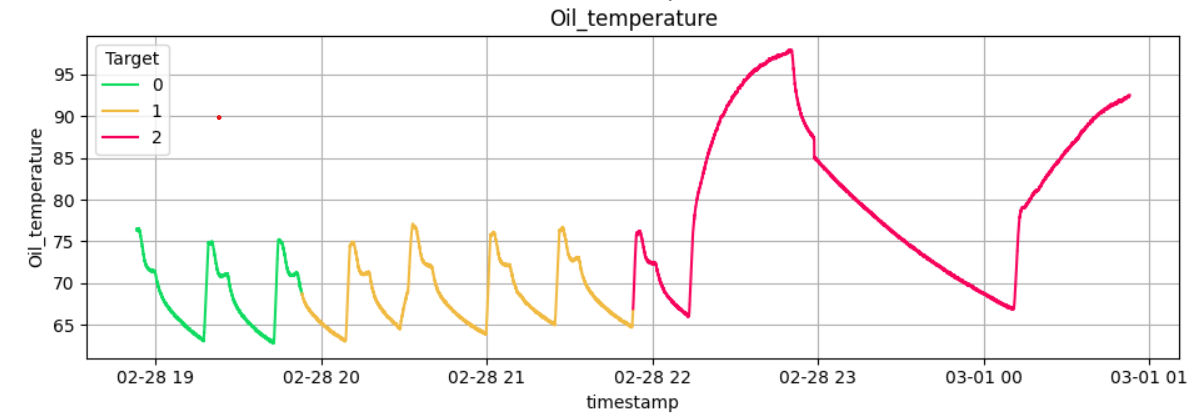
\includegraphics[width=1\textwidth]{EDA_oil.png}
    \caption{Oil tempreture increases before failure}
    \label{fig:Oil temp}
\end{figure}

There is also an increase in reservoirs prior to failure, however this effect is only seen in before the first failure and not before any other ones. which may related to component which is likely to fail this is one of the other tasks mentioned in the dataset \cite{Veloso2022}. See figure 3. \\

Our exploration of the dataset involved generating a correlation matrix, revealing several valuable insights. Notably, there exists a slight negative correlation between the Reservoirs variable and the target variable. Additionally, our analysis uncovered instances of multicollinearity within the dataset. example, we observed a negative correlation between the 'comp' variable and 'DV electric,' as well as between 'DV electric' and 'MPG' this would limit the performance of linear models, such as linear regression for RUL estimation. See figure 2 for more info.\\

It is essential to recognize that the exploratory data analysis (EDA) conducted in our study primarily encompasses fundamental analyses. The correlation matrix, for instance, exclusively reveals linear relationships, and the individual plots illustrate the influence of a single variable on the target variable. Given the substantial dimensionality of the data, comprehensively studying the complex interactions among variables becomes exceedingly challenging. \\

\begin{figure}
    \centering
    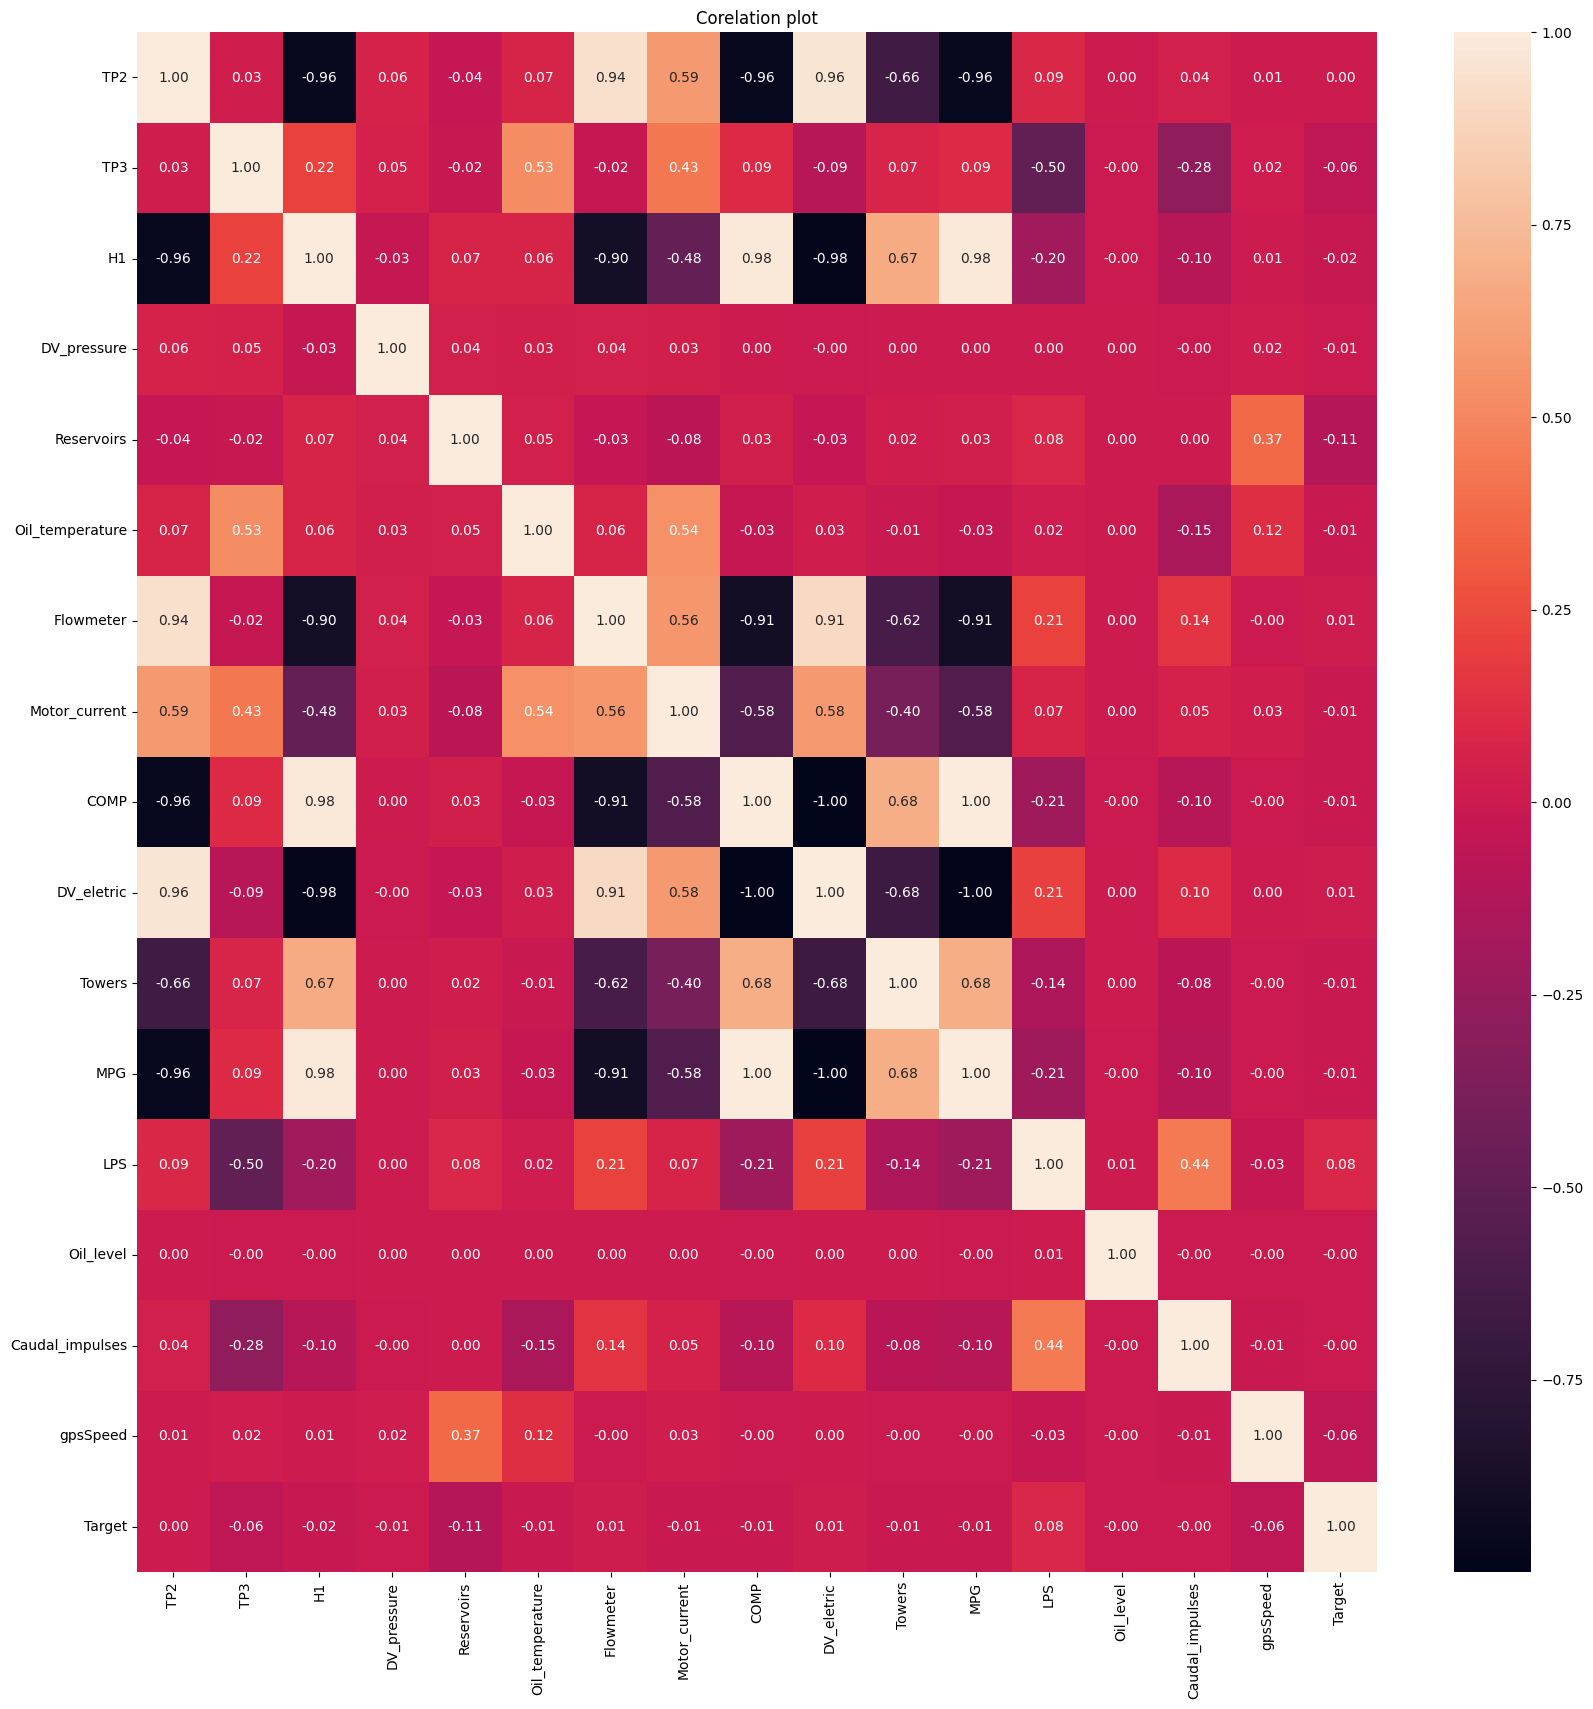
\includegraphics[width=1\linewidth]{cm.png}
    \caption{Plotting the corelation matrix}
    \label{fig:Corealtions}
\end{figure}

\begin{figure}
    \centering
    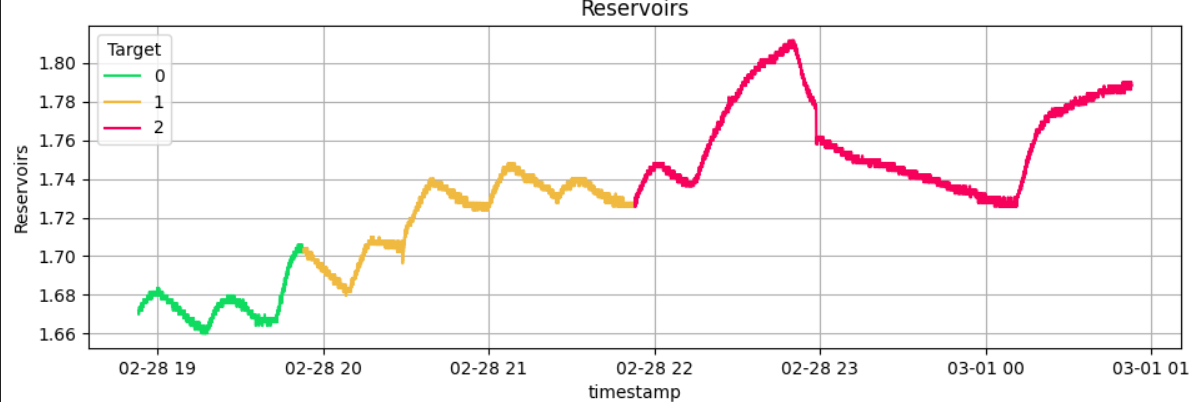
\includegraphics[width=1\linewidth]{EDA_Res.png}
    \caption{Enter Caption}
    \label{fig:enter-label}
\end{figure}

\section{Machine Learning for Failure Prediction}

As mentioned in the abstract, the comparative analysis will encompass several machine learning (ML) models and deep learning models. It is important to note that all figures presented in this study are computed using the test subset of the resampled data. Specifically, 30\% of the entire resampled dataset was designated for testing purposes. Furthermore a random seed of 42 was employed to ensure consistency in the selection of the test data. \\

Prior to delving into the model evaluations and results, it is imperative to establish a theoretical baseline. This baseline ensures that the models have learned meaningful patterns. \\

We three classes, each having approximately equal instances after resampling, thus we can reasonably assume that the probabilities of encountering each class are roughly equal, denoted as $P(Class_1) \approx P(Class_2) \approx P(Class_3)$. therefore, a model making random guesses would have an expected accuracy of 0.33, as it should have a $\frac{1}{3}$ chance of correctly predicting the class. Therefore, any accuracy significantly surpassing 0.33 on the testing data would signify that the model has successfully identified discernible patterns and is not relying on random chance for predictions.\\

\subsection{Support Vector Machines}

\subsubsection{Background}

The Support Vector Machine (SVM) is a classification algorithm that seeks to delineate data points using a hyperplane. By default, SVM is utilized to establish a linear decision boundary. However, through using the kernel trick, where a kernel transformation is applied to all data points before training the SVM, enabling the model to learn non-linear decision boundaries \cite{Geron2019}. For this problem we are using Gaussian RBF kernel defined as follows:

\begin{equation}
    \phi_\gamma(x, l) = \exp (-\gamma \|x + l\|)
\end{equation}

In the absence of a kernel, the SVM classifies data points based on a decision function, which is defined as follows:

\begin{equation}
\hat{y} =
    \begin{cases}
        0 & \text{if } w^Tx + b < 0\\
        1 & \text{if } w^Tx + b \geq 0
    \end{cases}
\end{equation}

Where the weight vector $w$ controls the width of the decision boundary, the smaller the value of $w$ the larger the decision boundary, thus we would like to minimize $\|w\|$. However, if we also want to avoid
any margin violation (hard margin), then we need the decision function to be greater
than 1 for all positive training instances, and lower than –1 for negative training
instances. This denotes a Hard Margin SVM.\\

Typically, two types of SVMs are employed: hard margin and soft margin SVMs. In a hard margin SVM, no data points are permitted within the margin. In contrast, a soft margin SVM allows for data points to be situated within the margin, and the extent to which this is allowed is regulated by a hyperparameter denoted as $C$ A smaller value of $C$ enforces a stricter margin, and $C = 0$ signifies a hard margin, where no points are permitted within the margin \cite{Geron2019}. In your specific case, you have chosen $C = 1$. Hard margin SVM are more prone to overfitting. To train a softmargin SVM we generally add a slack variable to the minimization equation.

\subsubsection{Results}

\begin{table}[htbp]
\centering
\caption{SVM Results}
\begin{tabular}{|l|lll|}
\hline
                    & \multicolumn{1}{l|}{\textbf{Normal}} & \multicolumn{1}{l|}{\textbf{Pre Failure}} & \textbf{Failure} \\ \hline
\textbf{Precision}  & \multicolumn{1}{l|}{0.55}            & \multicolumn{1}{l|}{0.60}                 & 0.52             \\ \hline
\textbf{Recall}     & \multicolumn{1}{l|}{0.62}            & \multicolumn{1}{l|}{0.62}                 & 0.36             \\ \hline
\textbf{F1 - Score} & \multicolumn{1}{l|}{0.58}            & \multicolumn{1}{l|}{0.61}                 & 0.43             \\ \hline
\textbf{Accuracy}   & \multicolumn{3}{r|}{0.57}                                                                           \\ \hline
\end{tabular}
\end{table}

The SVM model, without any hyperparameter optimization, has the worst performance, with an accuracy of 57\%. However this accuracy is still higher than the theoretical baseline of 33.33\% established at the beginning of Section 4. which means even this model is learning some pattern.\\

In terms of precision for class 1 (Pre-Failure), the SVM achieved a precision of 0.6, indicating that it correctly classifies 60\% of instances as pre-failure. This performance is particularly useful for us.\\

It's worth noting that the SVM appeared to struggle with distinguishing between normal and pre-failure states, with a misclassification rate of approximately 32\%. Additionally, it exhibited limited success in correctly predicting actual failure cases, achieving a correct prediction rate of only about 36\%.\\

These observations are supported by the confusion matrix presented below, which highlights the model's performance with respect to different classes. \\

\begin{align*}
\begin{bmatrix}
0.61969674 & 0.26742227 & 0.11288099 \\
0.32976412 & 0.61530106 & 0.05493482 \\
0.37874659 & 0.26006661 & 0.3611868 \\
\end{bmatrix}
\end{align*}

\subsection{Decision Trees}
\subsubsection{Background}

A decision tree is a widely used machine learning algorithm for classification tasks. It takes the form of a tree-like structure, where internal nodes represent decisions or tests based on input features, branches represent the outcomes of these decisions or tests, and leaf nodes signify class labels assigned to data instances.\\

It's essential to emphasize that, in theory, finding the most optimal decision tree is an NP-Complete problem. This means that, as the size and complexity of the dataset and the tree structure increase, the computational resources required to find the best tree become prohibitively large. NP-Complete problems are a class of problems for which no efficient polynomial time algorithm exists to find the exact optimal solution, making it necessary to rely on heuristics and approximations when building decision trees for practical applications \cite{laurent1976}.\\

Decision trees can be trained using various algorithms, and among them are CART (Classification and Regression Tree) and ID3 (Iterative Dichotomiser 3). For this study, the decision tree model will be constructed using the CART algorithm which has a cost function given by the following equation:

\begin{equation}
    J(k, t_k) = \frac{m_{left}}{m} \cdot G_{left} + \frac{m_{right}}{m} \cdot G_{right}
\end{equation}

Where $G_{left/right}$ is the Gini impurity and $m_{left/right}$ is the number of instances on left or right.\\

Gini Impurity is defined as follows:
\begin{equation}
    G_i = 1 - \sum_{k = 1}^{n}{P_{(i,k)}^2}
\end{equation}

Where $P_{(i,k)}$ is  is the ratio of class k instances among the training instances in the ith node

\subsubsection{Results}

\begin{table}[htbp]
\centering
\caption{Decision Tree Results}
\begin{tabular}{|l|lll|}
\hline
                    & \multicolumn{1}{l|}{\textbf{Normal}} & \multicolumn{1}{l|}{\textbf{Pre Failure}} & \textbf{Failure} \\ \hline
\textbf{Precision}  & \multicolumn{1}{l|}{0.70}            & \multicolumn{1}{l|}{0.69}                 & 0.51             \\ \hline
\textbf{Recall}     & \multicolumn{1}{l|}{0.68}            & \multicolumn{1}{l|}{0.70}                 & 0.52             \\ \hline
\textbf{F1 - Score} & \multicolumn{1}{l|}{0.69}            & \multicolumn{1}{l|}{0.70}                 & 0.52             \\ \hline
\textbf{Accuracy}   & \multicolumn{3}{r|}{0.66}                                                                           \\ \hline
\end{tabular}
\end{table}

The decision tree model represents an improvement over the SVM, achieving an accuracy of 66\%. The precision for pre-failure cases has also seen a substantial increase, reaching 69\%. Despite these improvements, the decision tree still faces challenges in reliably predicting failure cases. However, it's an improvement of almost 17\% compared to the SVM. \\

Additionally, the decision tree model demonstrates superior computational efficiency we will go over the computation complexity of the tested algorithms later, particularly for large datasets. It's important to mention that during hyperparameter tuning, different criteria were explored, including log\_loss, entropy, and Gini impurity, but the impact on model performance was relatively minor.\\

The confusion Matrix for the decision tree was as follows:

\begin{align*}
\begin{bmatrix}
0.68019605 & 0.18456119 & 0.13524276 \\
0.18171943 & 0.70251397 & 0.1157666 \\
0.22615804 & 0.25158946 & 0.5222525 \\
\end{bmatrix}
\end{align*}

\subsection{Random Forest}
\subsubsection{Background}

The Random Forest algorithm represents an improvement over  decision trees classifier. It is classified as an ensemble technique, which means it uses predictions from multiple models. Specifically, the Random Forest algorithm involves training a "forest" of numerous decision tree classifiers. In this instance, 100 different decision trees are used. During inference, the algorithm determines the most common class among the predictions.

\subsubsection{Results}

\begin{table}[htbp]
\centering
\caption{Random Forest Results}
\begin{tabular}{|l|lll|}
\hline
                    & \multicolumn{1}{l|}{\textbf{Normal}} & \multicolumn{1}{l|}{\textbf{Pre Failure}} & \textbf{Failure} \\ \hline
\textbf{Precision}  & \multicolumn{1}{l|}{0.73}            & \multicolumn{1}{l|}{0.69}                 & 0.70             \\ \hline
\textbf{Recall}     & \multicolumn{1}{l|}{0.72}            & \multicolumn{1}{l|}{0.78}                 & 0.54             \\ \hline
\textbf{F1 - Score} & \multicolumn{1}{l|}{0.72}            & \multicolumn{1}{l|}{0.73}                 & 0.61             \\ \hline
\textbf{Accuracy}   & \multicolumn{3}{r|}{0.70}                                                                           \\ \hline
\end{tabular}
\end{table}

The Random Forest indeed offers improvements over decision trees in various aspects. It has shown an increase in accuracy, precision, and recall.\\

During the hyperparameter optimization phase, a slight accuracy increase of 1\% was achieved by experimenting with different criteria, such as entropy.

\subsection{Neural Networks}
\subsubsection{Background}

Neural networks serve as the initial deep learning model to be applied in our study. They are fundamental examples of deep learning models neural networks are inspired by the structure of the human brain they can be conceptualized as a series of interconnected layers \cite{Goodfellow2016}.\\ 

Each layer can be viewed as an operation that applies a function to its input. This function typically involves various parameters that can be adjusted during training, these layers are usually followed by an activation function which is a non linear transformation applied to the output of a layer, this is usually done to allow the neural network to learn more complicated patterns, similar to the kernel trick used in SVMs \cite{Goodfellow2016}. \\

in our case this function is a Linear Layer followed by a hyperbolic tangent (tanh) activation function given by the following equation:

\begin{equation}
    f(x) = tanh(x \cdot w^T + b)
\end{equation}

Where $w$ and $b$ are the parameters of the layer. \\

In our study we decided to use the following neural Network architecture:\\

\begin{figure}[ht]
    \centering
    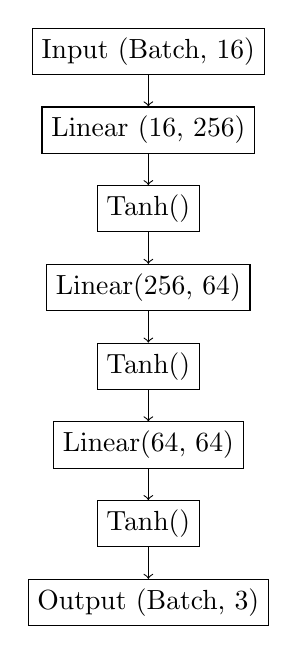
\begin{tikzpicture}[node distance=1cm]
        \node (input) [draw, rectangle] {Input (Batch, 16)};
        \node (l1) [draw, rectangle, below of=input] {Linear (16, 256)};
        \node (hidden1) [draw, rectangle, below of=l1] {Tanh()};
        \node (hidden2) [draw, rectangle, below of=hidden1] {Linear(256, 64)};
        \node (hidden3) [draw, rectangle, below of=hidden2] {Tanh()};
        \node (hidden4) [draw, rectangle, below of=hidden3] {Linear(64, 64)};
        \node (output) [draw, rectangle, below of=hidden4] {Tanh()};
        \node (caption) [draw, rectangle, below of=output] {Output (Batch, 3)};

        \draw[->] (input) -- (l1);
        \draw[->] (l1) -- (hidden1);
        \draw[->] (hidden1) -- (hidden2);
        \draw[->] (hidden2) -- (hidden3);
        \draw[->] (hidden3) -- (hidden4);
        \draw[->] (hidden4) -- (output);
        \draw[->] (output) -- (caption);
    \end{tikzpicture}
    \caption{Neural Network Architecture}
\end{figure}

The output of the model will be a 3-d Vector representing the probability of each class, $x_i = P(class_i)$. we will ensure these vectors sum to 1 by making use of the softmax function.\\

\begin{equation}
    \text{softmax}(x) = \frac{\exp{x_i}}{\sum_i{\exp x_i}}
\end{equation}

Neural networks are commonly trained in batches of input data. This batching approach is primarily adopted for efficiency purposes, as GPUs which are used in training neural network models excel at parallel processing. In our study we found that a batch size of 32 worked best for our system. \\

In essence, the objective of a neural network is to discover the optimal values for these parameters, or trying to find the most suitable values within a reasonable time frame. In order to accomplish this there needs to be some measure of the quality of the output produced by the network, called a loss function.\\

In our case we would like the target class to have the highest probability, to do this we make use of the cross entropy loss function, in particular the categorical cross entropy loss function defined as follows:

\begin{align}
    w_y \in \mathbb{R}^C, w_i &= \begin{cases}
    1 & \text{if } i = y\\
    0 & \text{otherwise}
\end{cases} \\
    L(x,y) &= -w_y\log{\text{softmax}(x)} \\
    &= -w_y\log{\frac{\exp{x_i}}{\sum_i{\exp x_i}}}
\end{align}

Training a neural network involves the use of an optimizer, which plays a pivotal role in iteratively updating the values of model parameters. The optimizer does this by utilizing the derivatives of the loss function with respect to each parameter, and this process is repeated until the model converges to a local minimum, optimizing its performance.\\

Through hyperparameter optimization, it was determined that the AdamW optimizer, with a learning rate of 1e-3, yielded the best results. AdamW is a variant of the popular Adam optimizer \cite{loshchilov2019}.\\

A learning rate scheduler is employed in conjunction with the optimizer. This scheduler dynamically adjusts the learning rate during training. Specifically, it lowers the learning rate when the loss begins to plateau. This adaptive adjustment helps the model converge effectively.\\

Furthermore, an early stopping callback is used, primarily to reduce the risk of overfitting. Early stopping monitors the model's performance on a validation dataset and stops training when the performance ceases to improve or even deteriorates.

\subsubsection{Results}

\begin{table}[hbpt]
\caption{neural network result}
\centering
\begin{tabular}{|l|lll|}
\hline
                    & \multicolumn{1}{l|}{\textbf{Normal}} & \multicolumn{1}{l|}{\textbf{Pre Failure}} & \textbf{Failure} \\ \hline
\textbf{Precision}  & \multicolumn{1}{l|}{0.78}            & \multicolumn{1}{l|}{0.75}                 & 0.74             \\ \hline
\textbf{Recall}     & \multicolumn{1}{l|}{0.76}            & \multicolumn{1}{l|}{0.87}                 & 0.57             \\ \hline
\textbf{F1 - Score} & \multicolumn{1}{l|}{0.77}            & \multicolumn{1}{l|}{0.80}                 & 0.64             \\ \hline
\textbf{Accuracy}   & \multicolumn{3}{r|}{0.76}                                                                           \\ \hline
\end{tabular}
\end{table}

The neural network has demonstrated remarkable performance, surpassing previous machine learning approaches by a significant margin across all evaluation metrics. The accuracy stands out with a notable 6\% improvement over the Random Forest model. The true positive rate, or recall, for pre-failure cases is an impressive 87\%, signifying that 87\% of actual pre-failure cases are correctly identified.\\

However, it's important to acknowledge that comes with trade-offs. Training the neural network takes longer than decision trees and Random Forest, even when utilizing a CUDA-enabled GPU in our case Nvidia RTX 3050. Moreover, deployment of the model may present challenges, particularly when access to a CUDA-enabled GPU is not readily available, such as on edge devices like sensors.\\

To address these concerns, we explored the optimization of the model using the PyTorch JIT (Just-In-Time) compiler. Which claims to increase performance on edge devices, However real world testing of this claim is still to be conducted. Additionally, it's worth considering the capabilities of modern CPUs, which can execute relatively small models efficiently, providing a viable alternative when GPU access is limited. Extensive testing on CPUs is recommended to ensure satisfactory performance in such scenarios before deployment.

\subsection{LSTM Networks}
\subsubsection{Background}

LSTM models, short for Long Short-Term Memory models, represent a category of deep learning architectures specialized in handling sequential data, such as text or time series data. They derive their roots from Recurrent Neural Networks (RNNs) but offer distinct advantages, particularly when dealing with sequences with large temporal dependencies. One advantage of LSTMs is their ability to mitigate the "vanishing gradients" issue, which is a common challenge encountered in training RNNs. The vanishing gradients problem refers to the diminishing influence of gradients during the training process especially when dealing with long sequences, hindering the network's ability to capture long-range dependencies effectively \cite{zhang2023}. \\

\begin{figure}
    \centering
    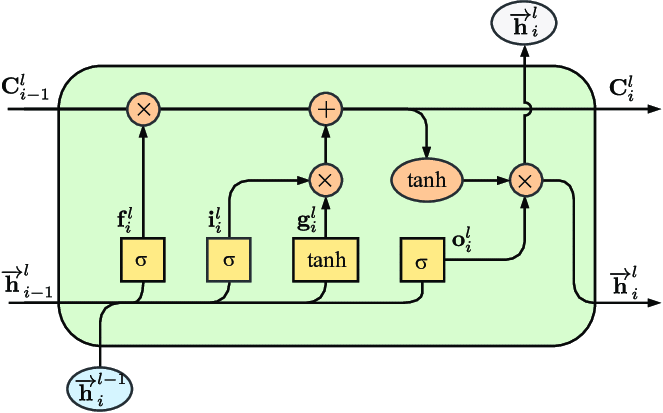
\includegraphics[width=0.5\linewidth]{LSTM.png}
    \caption{LSTM Cell Architecture}
    \label{fig:LSTM Diagram}
\end{figure}

In architectural terms, LSTMs exhibit similarities to standard RNNs, given their shared reliance on recurrent connections. However, LSTMs introduce a pivotal architectural element, the memory cell, which assumes the responsibility of preserving the network's long-term memory. This memory cell is equipped with four crucial gated components: the forget gate, input gate, input node, and output gate. \\

In Figure 2 the input is denoted $\Vec{h_i}$ the hidden unit of the previous layer (Like RNNs) is denoted $\vec{h_{i-1}}$ the forget gate is $f_i$ decicdes if the current memory state should be discarded or not, input gate is $i_i$, the input node is denoted $g_i$ and the output is denoted $o_i$ the $\times$ symbol means a hadamard or elementwise multiplication. and $\sigma$ denotes the sigmoid activation function defined as:\\

\begin{equation}
    \sigma(x) = \frac{1}{1+\exp(-x)}
\end{equation}

in terms of the implementation the gates G in an LSTM is similar to a linear layer with 2 inputs the current input $X$ and the output of previous timestep $H_{t-1}$ expressed as follows:

\begin{equation}
    G = \sigma(XW_g + H_{t-1}W_g + b)
\end{equation}

During each time step, LSTM cell returns both the current hidden state and memory cell state. This allows the stacking of LSTMs, which, can be used to create highly intricate architectures, in our study we stack 3 LSTMs.\\

\subsubsection{Data preprocessing for the LSTM}

The preparation of data for LSTM models in the context of sequential data can indeed present significant challenges. In our study, we made a specific choice regarding the context length, opting for a value of 84. While this choice may appear somewhat arbitrary, it holds significance as it represents a multiple of the total number of records within our dataset. This selection strikes a balance between avoiding a context length that is overly small, as it might hinder the LSTM's capacity to capture time-based patterns, and steering clear of a context length that is too large, which would increase the time taken to train the model. we will refer to this context lenght as $s = 84$ for this section.\\

To process the dataset we begin with the base classification dataset that we created for all classification task this dataset has the $n$ = 10.7 Million rows (1.07 crores) and $m$ = 16 columns, the first step is creating the Input the $X$ Matrix. then we split the matrix into chunks of $s$ (84 in our case) which creates a 3rd order tensor with the shape $\left[ \frac{n}{s}, s, m - 1 \right]$.\\

The next step in data preparation is to create the target column this is what the model will try to predict. creating the target column is rather simple and we do this selecting the value of the target column at the end of each sequence. 

\subsubsection{Results}

A significant challenge inherent to LSTM models pertains to the nature of the input data. Given that the input data is structured as a 3rd order tensor, the process of resampling this data becomes notably complex. Traditional machine learning libraries commonly utilized are not well-equipped to handle intricate datasets like 3rd order tensors. Consequently, the development of custom algorithms is necessitated to address this issue. It's crucial to note that, unlike our previous approaches, the results obtained for LSTM models were attained without the use of data balancing techniques. This means that the results should be tested when practical performance of an LSTM-based system is considered for production. It's worth mentioning that a similar challenge would also be encountered with any Convolutional Neural Network (CNN) based approach, as CNNs require image inputs, which, too, are represented as higher order tensors.\\

However to address this issue we did consider using a balanced accuracy metric which uses the number of instances of a class when determining the accuracy. this metric is not influenced by the number of instances in a class and the accuracy does not change much when the model predicts a majority class correctly. A good explanation on balanced accuracy can be found in a blog by Olugbenga for NeptuneAI, in their blog the go over how balanced accuracy works and the advantages this metric. \cite{Olugbenga2023}.\\

\begin{table}[htbp]
\caption{LSTM Results}
\centering
\begin{tabular}{|l|lll|}
\hline
                    & \multicolumn{1}{l|}{\textbf{Normal}} & \multicolumn{1}{l|}{\textbf{Pre Failure}} & \textbf{Failure} \\ \hline
\textbf{Precision}  & \multicolumn{1}{l|}{1}               & \multicolumn{1}{l|}{0}                    & 0.02             \\ \hline
\textbf{Recall}     & \multicolumn{1}{l|}{0.97}            & \multicolumn{1}{l|}{0}                    & 1                \\ \hline
\textbf{F1 - Score} & \multicolumn{1}{l|}{0.98}            & \multicolumn{1}{l|}{0}                    & 0.03             \\ \hline
\textbf{Accuracy}   & \multicolumn{3}{r|}{0.74}                                                                           \\ \hline
\end{tabular}
\end{table}

Table 7 provides a clear indication that this particular model predominantly classifies all data points as normal, with minimal effort to identify failure cases. Its performance in this regard is notably poor, as evidenced by the extremely low F1 Score of 0.03. As mentioned previously, the deployment of an LSTM-based model necessitates a thorough investigation and refinement before considering practical implementation. In terms of the balanced accuracy it is better than Random Forest but worse than the neural network.


\section{Deployment and future scope}
As we previously mention, one of the objectives of our study is to not only evaluate these models but also offer guidance on their practical deployment in production settings. To accomplish this, we have implemented an API, which stands for Application Programming Interface. An API is a set of rules and protocols that allows different software applications to communicate and interact with each other. In our case, this API is designed to leverage one of the models, specifically the neural network, for making real-time predictions on incoming data.\\

It's important to note that our approach is highly versatile and extensible. While we have chosen to utilize the neural network for this purpose, we have designed the system in a manner that allows for use with other models if desired. This flexibility ensures that the API can accommodate a variety of machine learning models, enabling adaptability to specific needs and requirements in different production scenarios.\\

In addition to the model API, we strongly recommend implementing a separate API dedicated to database functionality. This approach offers multiple advantages. Firstly, it enables the adoption of a microservice architecture, which is beneficial because it allows for individual scalability of different components according to specific needs \cite{Patel2021}. \\

The database API, for instance, primarily demands increased storage resources rather than computational power. Consequently, you can deploy cloud instances with greater storage capacity to run the database service, while, in contrast, the model API might require enhanced computational resources and, potentially, a CUDA-compatible GPU for efficient execution.\\

Secondly, this separation of concerns is highly advantageous. It ensures that the ML model remains agnostic to the database schema, which not only enhances modularity but also simplifies maintenance and future modifications, we facilitate easier development, testing, and maintenance of each component, contributing to the overall robustness and flexibility of the system. \\

Figure 3 shows the basic architecture diagram we have implemented in this project, however we aknowledge the need of projects differ but these are some recommendations that we make, when deploying this model

\begin{figure}
    \centering
    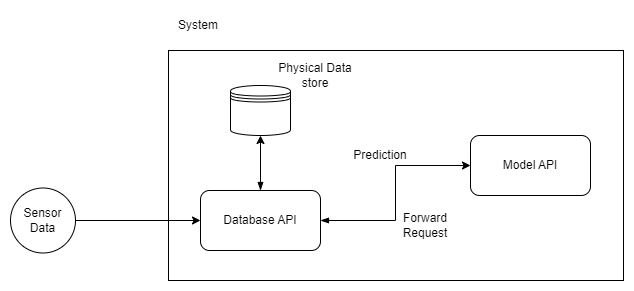
\includegraphics[width=1\linewidth]{architecture_basic.png}
    \caption{basic architecture}
    \label{fig:architecture}
\end{figure}

\section{Conclusion}

\begin{table}[htbp]
\caption{Results summary of all models}
\centering
\begin{tabular}{l|c|c|c|}
\cline{2-4}
                                             & \multicolumn{1}{l|}{Accuracy} & \multicolumn{1}{l|}{Precision (Class 2)} & \multicolumn{1}{l|}{Recall (Class 2)} \\ \hline
\multicolumn{1}{|l|}{SVM}                    & 0.57                          & 0.60                                     & 0.62                                  \\
\multicolumn{1}{|l|}{Decision Tree}          & 0.66                          & 0.69                                     & 0.70                                  \\
\multicolumn{1}{|l|}{Random Forest}          & 0.70                          & \textit{0.69}                            & 0.78                                  \\
\multicolumn{1}{|l|}{Neural Network (Adam)}  & 0.72                          & 0.67                                     & \textbf{0.91}                         \\
\multicolumn{1}{|l|}{Neural Network (AdamW)} & \textbf{0.76}                 & \textbf{0.75}                            & \textit{0.87}                         \\
\multicolumn{1}{|l|}{LSTM}                   & 0.74*                         & -                                    & -                                 \\ \hline
\end{tabular}
\end{table}

Table 8 provides a comprehensive summary of all the models that were evaluated during our research, along with the key metrics that were important for our investigation. In our case, where the primary objective is to predict failures in advance, we specifically focused on precision and recall for the pre-failure class.\\

Precision signifies the proportion of positive cases that the model correctly predicts. In other words, if the model has a precision of "p," it means that when the model signals a pre-failure event, it is correct approximately "p" percent.\\

Recall, on the other hand, is defined as the proportion of all actual positives that the model successfully identifies. A recall value of "r" implies that our model accurately predicts "r" percent of pre-failure events.\\

It's crucial to understand the trade-off between precision and recall. As one metric increases, the other tends to decrease. Therefore, when deploying our model, it becomes necessary to establish a threshold according to the specific project requirements. If we opt for a high recall setup, we increase the likelihood of correctly identifying all pre-failure cases, but this may also lead to more false positives. Conversely, a high precision indicates that when the model predicts a pre-failure event, it is highly likely to be correct, but there's a risk of missing some pre-failure cases.\\

The choice of a model for deployment should consider the project's particular needs, and the threshold for classification can be appropriately set to prioritize either precision or recall. In Table 8, we have highlighted the models with the best precision and best recall in bold, and the second-best models in italics, allowing for flexibility in model selection based on the project's specific requirements. \\

From this study we have found that simple neural network based algorithms work best for this classification problem however a good alternative could be to use random forest if computational resources are a limitation when it comes to deployment. \\

Our study does not fully explore utilise the temporal relationships in the data and the true capabilities of the LSTM model due to the difficulty in balancing the data. \\

Another aspect which could be explored in the future is the use of transformer based models for predicting failures as well as security concerns when deploying these model, with the key question being how we can ensure that data is sent by a valid sensor on the network.

\newpage

\bibliographystyle{IEEEtran}
\bibliography{metropt}

\end{document}
